\documentclass[11pt]{article}
\usepackage[a4paper, margin=2cm]{geometry}
\usepackage[utf8]{inputenc}
\usepackage{amsmath}
\usepackage{amsfonts}
\usepackage{graphicx}\graphicspath{{images/}}
\usepackage{hyperref}
\usepackage{xcolor}

\begin{document}
\pagenumbering{gobble}

\begin{titlepage}
   \begin{center}
       \vspace*{6cm}
		
       \begin{large}\textbf{MXB326 Group Project - Reservoir Simulation}\end{large}

       \vspace{0.5cm}
        MXB326\_23se1 Computational Methods 2\\
        Due 26-05-2023
            
       \vspace{1.5cm}

       \textbf{Group 5: Benjamin Elliott, Christopher Deveney, Kye Miethke}

       \vfill
            
       MXB326\_23se1 Computational Methods 2\\
       Queensland University of Technology\\
       Semester 1 2023
            
   \end{center}
\end{titlepage}
\newpage

%================================== Outline ==================================%

\tableofcontents
\newpage
\pagenumbering{arabic}


\section{Introduction}
%================================== Introduction ==================================%
Oil is a natural resource which is used abundantly in modern society. Necessary for the creation of fuels which transport us around the world, to materials in products we use hundreds of times a day, and many applications in between, it is no stretch to say that civilisation as we know it relies on oil. But the production of oil can be a slow and costly process. One method commonly used in the oil industry to improve production is called water-flooding. This processes uses the injection of water into the porous rock structure of an oil reservoir to increase the pressure, driving more oil out. Modelling this process mathematically is a key interest of a field of research known as reservoir engineering, and is of vital importance to ensure that the process of water-flooding runs smoothly.\\

This modelling, involving the simultaneous flow of two viscous fluids through a horizontal reservoir in three dimensions, is quite complex. Fortunately, the model can be substantially simplified when considering a homogeneous, one-dimensional reservoir. This simplification in turn reduces what would be a coupled system of partial differential equations into a single, one-dimensional PDE. To describe the mechanics of the system, the conservation of mass of oil and water assuming immiscibility and incompressibility, are given by the transport equations:
\begin{eqnarray}
\phi\frac{\partial S_w}{\partial t} + \frac{\partial q_w}{\partial x} = 0\\
\phi\frac{\partial S_o}{\partial t} + \frac{\partial q_o}{\partial x} = 0
\end{eqnarray}
In this system, $\phi$ indicates how porous the medium of the reservoir is, and $S_w$ and $q_w$, $S_o$ and $q_o$ indicate the saturation and flow rate of the water and oil respectively. We relate the pressure in each fluid as the capillary pressure: $P_c = p_o-p_w$, and assume that the capillary pressure is positive. Furthermore, the saturations of the oil and water can be related as $S_w +S_o = 1$, allowing a single saturation, $S=S_o$ to be the sole variable to be modelled. Also defined are the minimum, irreducible saturations $S_{or}$ and $S_{wr}$.\\

For a comprehensive description of the mathematical system, it is also necessary to define the conditions at the boundaries of the domain.
\begin{figure}[!h]
\centering
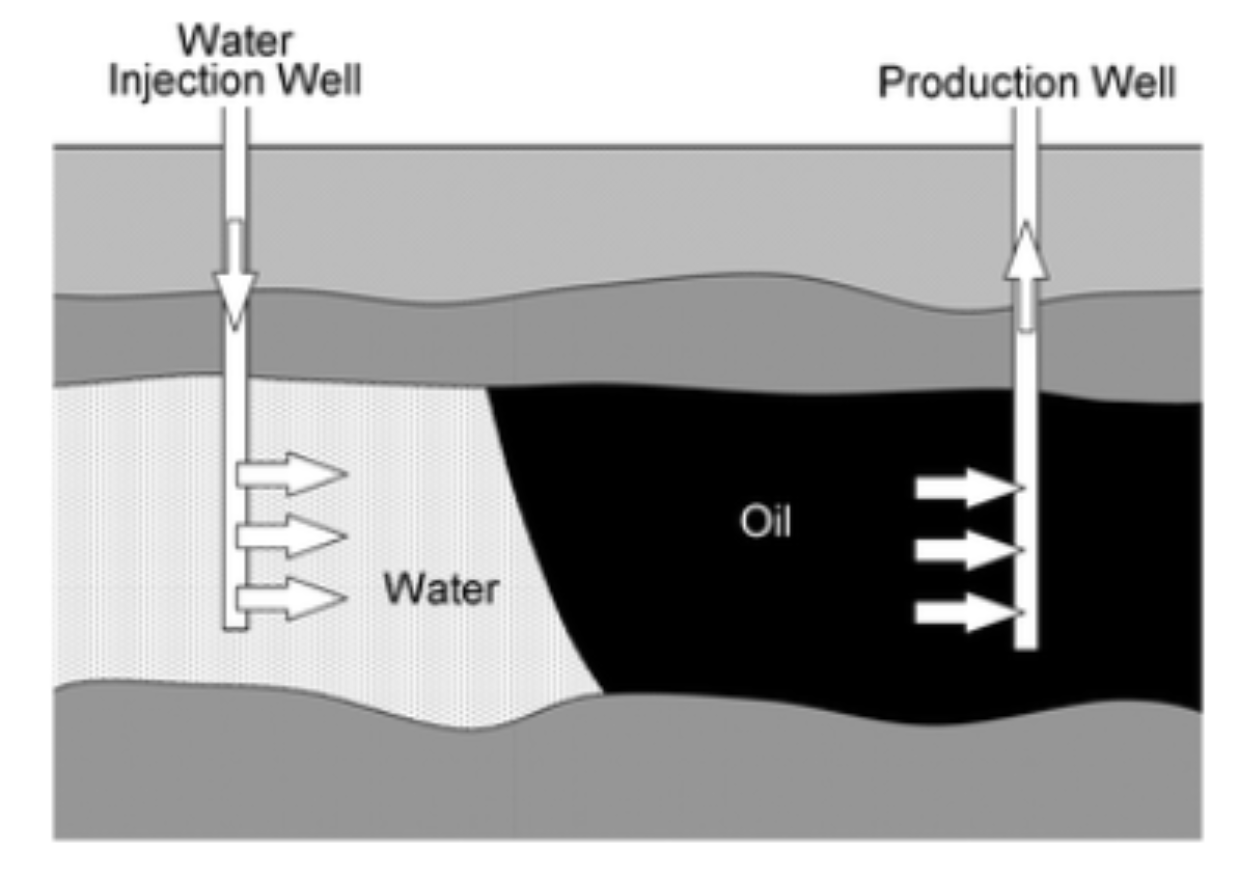
\includegraphics[width=0.4\textwidth]{injectionschematic.png}
\caption{Schematic of the oil injection process.}
\end{figure}
Figure 1 demonstrates the domain of the problem. Assuming a constant injection of water at $x=0$ at rate $q$:
\begin{eqnarray}
q_w(0,t) = q\quad\text{and}\quad q_o(0,t) = 0
\end{eqnarray}
And assuming oil saturation begins at its maximum value:
\begin{eqnarray}
S(x,0)=1-S_{wr}
\end{eqnarray}
Finally, assuming a semi-infinite reservoir:
\begin{eqnarray}
\lim_{x\to\infty} S(x,t) = 1-S_{wr}
\end{eqnarray}
For an efficient and cost-effective water-flooding operation, it is critical to prevent the water from mixing with the oil in the well-bore (extraction point). We thus define the breakthrough time as $T_B = 1-S_{or}-S_{wr}$, the time taken for the water to reach the well-bore during the water-flooding. Specification of a suitable injection rate $q$ is capable of preventing this issue from arising.\\

This report contains a pilot study of the simplified system above, including a mathematical model with a semi-analytic solution and a numerical solution. These solutions will be analysed thoroughly, with the goal of demonstrating the capability of a fully detailed study in the future.

\smallbreak
\section{Mathematical Model}
%================================== Mathematical Model ==================================%
It is possible to derive an exact solution for the system described above using methods from \emph{Fokas and Yortsos}, in the case of constant injection rates when the water to oil viscosity ratio $F$ has the form
\begin{eqnarray}
F=\frac{1-S_{wr}+\frac{\gamma}{\beta}}{S_{or}+\frac{\gamma}{\beta}}
\end{eqnarray}

Applying this, the following one-dimensional initial boundary value problem can be derived for the oil saturation:
\begin{eqnarray}
\frac{\partial S}{\partial t} = \frac{\partial}{\partial x} \big[g(S)\frac{\partial S}{\partial x} + f(S)\big],\\
S(x,0)=1-S_{wr},\\
\frac{\partial S}{\partial x}(0,t) = \frac{\alpha}{\beta}(\beta S(0,t)+\gamma) + \frac{\omega}{\beta}(\beta S(0,t)+\gamma)^2,\\
\lim_{x\to\infty}S(x,t)=1-S_{wr}.
\end{eqnarray}

By specifying $S_{wr}, S_{or}, F, \text{and} \beta$, the remaining parameters can be determined from (6) as well as the relations
\begin{eqnarray}
\frac{\alpha}{\beta^2}=-\frac{(S_{or}+\frac{\gamma}{\beta})(1-S_{wr}+\frac{\gamma}{\beta})}{1-S_{wr}-S_{or}},\\
\omega = \beta -\frac{\alpha}{\beta-\beta S_{wr}+\gamma}.
\end{eqnarray}
Using these equations, $\gamma$ can be found with equation (6), $\alpha$ with $\gamma$ and equation (11), and $\omega$ using the other two parameters with equation (12). This process has been implemented in the function \verb|paramsFunc|.\\

Furthermore, the functions $f(S)$ and $g(S)$, called the capillary-hydraulic properties of the fluid-porous system are given by
\begin{eqnarray*}
f(S) = \frac{\alpha}{\beta^2}\bigg[\frac{1}{1-S_{wr}+\frac{\gamma}{\beta}}-\frac{1}{S+\frac{\gamma}{\beta}}\bigg],\quad g(S)=\frac{1}{(\beta S+\gamma)^2}.
\end{eqnarray*}
These functions allow for an exactly solvable PDE (7), and also correspond to a physically meaningful model.

\smallbreak
\section{Semi-Analytical Solution}
%================================== Semi-Analytical Model ==================================%
A semi-analytical solution for (7) can be derived at discrete space $x_i$ and time $t_n$ by applying the spacial transformation 
\begin{eqnarray}
\tilde x = \int_0^x (\beta S(\xi,t)+\gamma)d\xi + \omega t,
\end{eqnarray}
This linearises the equation and yields the solution for $S$:
\begin{eqnarray}
S(x,t) = \frac{1}{\beta}\left[\frac{\alpha e^{\alpha x}}{\frac{\partial\phi}{\partial\tilde x}(\tilde x,t)}-\gamma\right],
\end{eqnarray}
where $\tilde x$ is the solution of $\phi(\tilde x,t)=e^{\alpha x}$ for a given $x$ and $t$. 
The solution of the nonlinear equation must be obtained using MATLAB's \verb|fzero| function. The MATLAB documentation for this function indicates that it is used to find the roots of nonlinear function. Specifically, for some input \verb|x = fzero(func, x0)|, \verb|x| will return a point where $\text{func}(x) = 0$. The \verb|fzero| function requires an initial guess $x_0$ such that $\text{func}(x_0) \approx 0$. An appropriate guess for each $i=1..N$ and $n=1..M$ can be found by evaluating (13) at $x=x_i$ and $t=t_{n-1}$. Let $\hat x$ indicate the approximate initial guess. Thus we have:
\begin{eqnarray}
\hat x_{i,n} = \left(\beta S(x_i, t_{n-1})+\gamma\right)x_i + \omega t_{n-1}
\end{eqnarray}

This results in an iterative process for the semi-analytical solution: for each $t_n$, solve for all $x_i$ using $S(x_i,t_{n-1})$. For the initial guess at $t=t_1$, the initial condition (8) is applied. This provides $\hat x$ for all $x_i$ at $t=t_1$:
\begin{eqnarray}
\hat x_{i,1} = \left[\beta (1-S_{wr})+\gamma\right]x_i
\end{eqnarray}
With an iterative solution defined and appropriate initial conditions, the solution can be straightforwardly determined using MATLAB. This solution is implemented in the MATLAB script \verb|semianalytic.m|, and produces the following result:
\begin{figure}[!h]
\centering
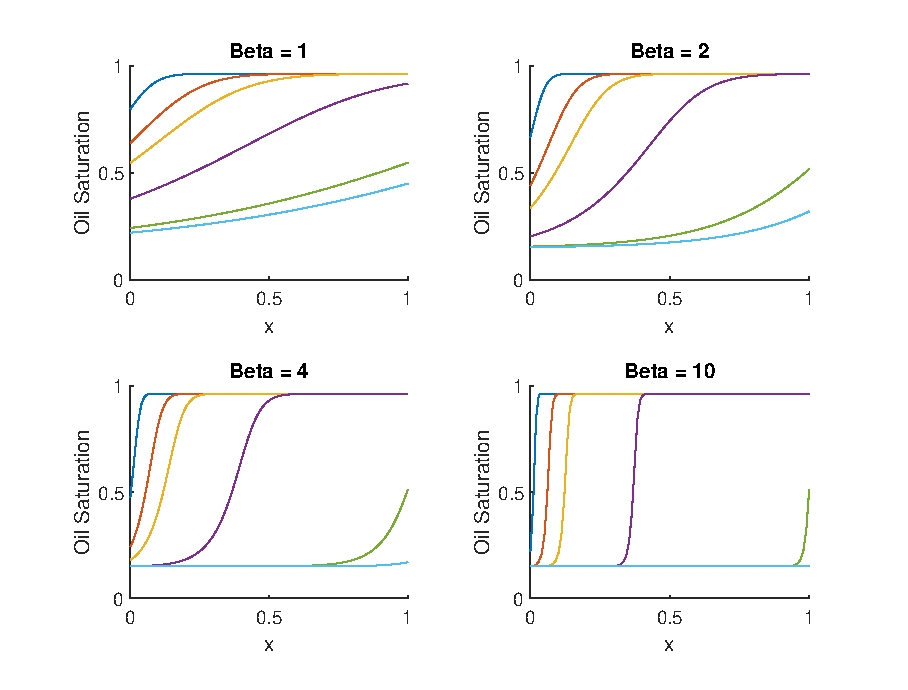
\includegraphics[width=0.8\textwidth]{semianalyticsolution.eps}
\caption{The semi analytical solution, plotted from $x=0$ to $x=1$ at $t=0.01, 0.05, 0.1, 0.3, 0.8125, 1$, for $\beta=1,2,4,10$.}
\end{figure}


\smallbreak
\section{Numerical Solution}
%================================== Numerical Solution ==================================%

\smallbreak
\section{Analysis and Findings}
%================================== Analysis and Findings ==================================%
\subsection{Comparison of semi-analytical solution and numerical solution}

\subsection{Average reservoir oil saturation}


\subsection{Computational efficiency analysis}

\subsection{Buckley-Leverett solution analysis}
For large $\beta$, the capillary forces are negligible when compared to the viscous forces. As a result, the method of characteristics can be used to obtain a simplified solution. The solution exhibits Buckley-Leverett shock front behaviour given by
\begin{eqnarray}
S(x,t) = \bigg\{
\begin{array}{lr}
S_{or}, &x<vt,\\
1-S_{wr}, &x>vt.
\end{array},\quad\text{where} \quad v = \frac{1}{1-S_{wr}-S_{or}}
\end{eqnarray}
This is implemented in MATLAB as the function \verb|BuckleyLeverett.m|. Plotting the Buckley-Leverett shock front against the semi-analytical solution with $\beta=10$, it can be seen that the semi-analytical solution does exhibit the shock front behaviour:

\begin{figure}[!h]
\centering
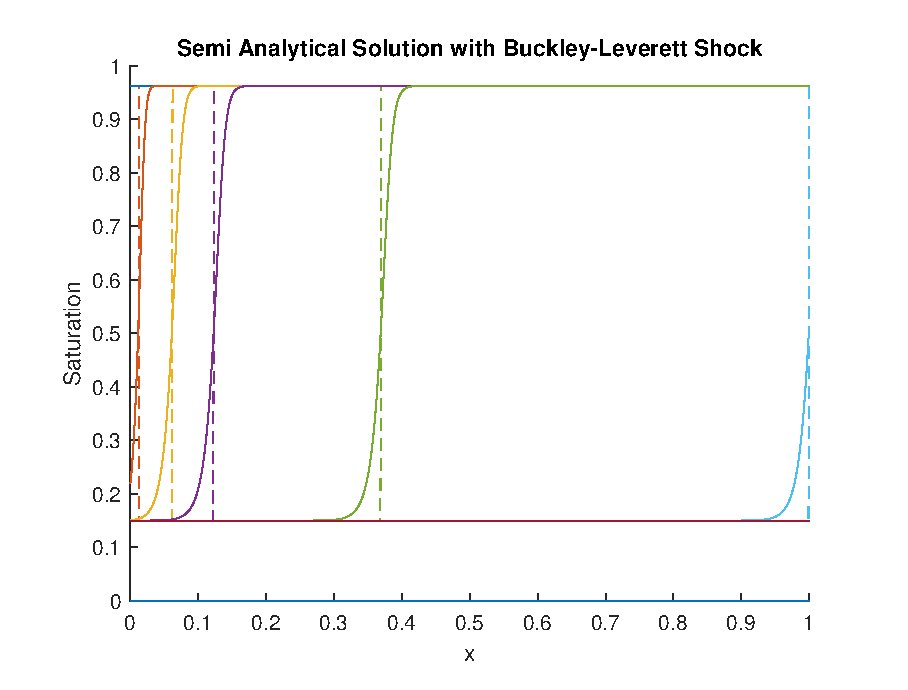
\includegraphics[width = 0.6\textwidth]{semianalytical-buckleyleverett.eps}
\caption{The semi-analytical solution with $\beta=10$ plotted against the Buckley-Leverett shock front.}
\end{figure}

Similarly for the numerical solution:\\


As has been observed in the plots previously, increases of $\beta$ correspond to increases of the slope of the front between the phases. As such, the shock front behaviour of becoming perfectly vertical as $\beta\to\infty$ is reasonable.

\subsection{Impact of different injection rates}
\smallbreak
\section{Conclusions}
%================================== Conclusions ==================================%

\smallbreak
\section{References}
%================================== References ==================================%

\newpage
\end{document}
